\section{Implementation of Perturb and Observe algorithm}\label{MPPTImplementation}

Due to the previous mentioned advantages of the Perturb and Observe (P\&O) algorithm it was decided to implement this commonly used control algorithm for tracking the MPP. The basic operation of the P\&O algorithm consists of perturbing the operating voltage of the PV module by means of the variation of the duty cycle of the DC-DC converter. After each perturbation the power generated by the PV module is measured (observed) and stored in order to compare it with the previous value of the power. Based on the result of the comparison the MPP can be tracked by deciding if in the next perturbation the module's voltage should be increased (decrease duty cycle) or decreased (increase duty cycle). 

There are different techniques for implement the P\&O algorithm according to the value of the variable controlled by the MPPT and also depending if the perturb value is fixed or variable \todo{REF to "Perturb and observe MPPT technique for PV based microgrids"}. The conventional P\&O algorithm uses a fixed perturb to generate a voltage or current reference signal for the outer control loop. The outer loop is usually a PI controller which controls the switching of the DC-DC converter. Another way of implementing the conventional P\&O algorithm is using an adaptive perturb by setting the initial perturbation to 10\% of the open-circuit voltage ($V_{oc}$). After each iteraction its value is decreased by 50\% until it reaches 0.5\%
of $V_{oc}$. A different technique consists of using the duty cycle of the converter as the variable controlled by the MPPT block and, therefore, avoiding the PI controller. As with the conventional P\&O method this technique can also be implemented using fix or variable perturb step \todo{REF to "Perturb and observe MPPT technique for PV based microgrids"}. 

The P\&O algorithm that will be implemented in this project is the modified version of the conventional one and using a variable perturb step. It was decided to directly control the duty cycle to simplify the control system as it is not necessary to implement the PI controller \todo{Are we going to implement the PI controller at some point??}. On the other hand, an adaptive perturb is selected instead of a fix one because if a small perturb step is implemented the MPPT takes longer time to reach the MPP, however, using a large perturb step the tracking would be faster but the oscillations around the MPP would be higher \todo{REF to "Perturb and observe MPPT technique for PV based microgrids"}. For this reason, it was decided to start with a perturbation step of 10\% of the $V_{oc}$ until the system detects the first MPP crossing \todo{check this with the final implementation in the lab?? delta D is 0.0122 for 0.45V increment/decrement}. At this point the perturbation step is iteractively reduced to half of its previous value in order to reach accurately the MPP with lower oscillations. Figure \ref{BD_POalgorithm} shows the implementation of the system in \textit{PLECS} including the MPPT controller unit which operates at a frequency of 100 Hz. 

\begin{figure}[H]
	\begin{center}
		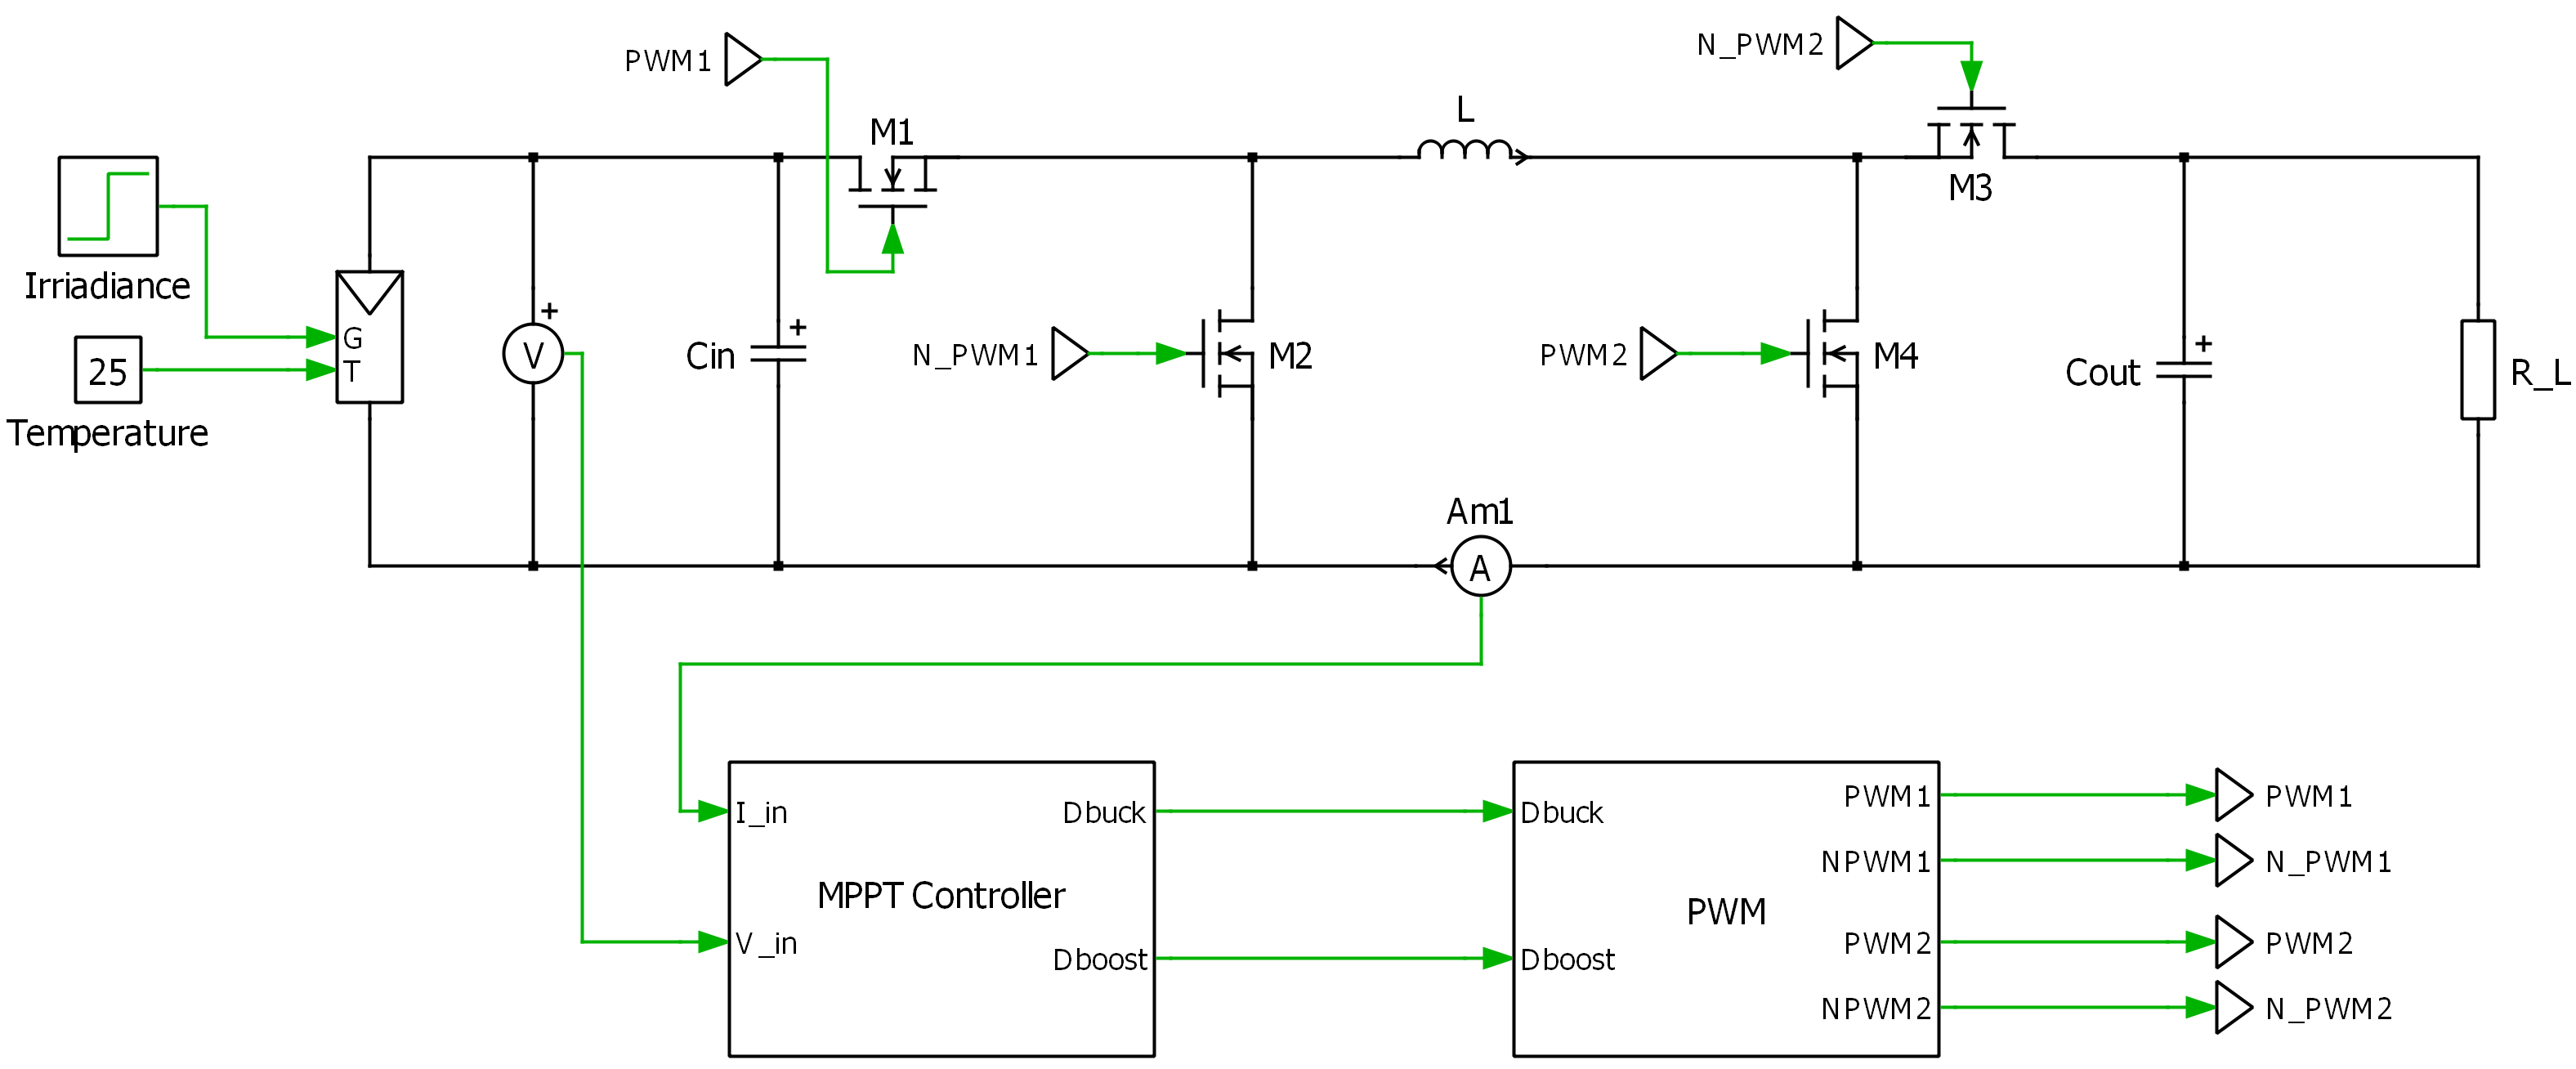
\includegraphics[width=\textwidth]{../Pictures/BD_implementation_POalgorithm}
		\caption{Block diagram of the system including the MPPT.}
		\label{BD_POalgorithm}
	\end{center}	
\end{figure}

From the previous figure it is observed that the output of the MPPT is a duty cycle which is send to another block called "Mode decision". This block is used to decide if the DC-DC converter operates in buck or in boost mode. The transfer function of the converter when it is operating in buck and in boost mode is shown in equations \ref{tfbuck} and \ref{tfboost}, respectively. Plotting this transfer functions in figure \ref{fig:tfmodes} and mapping them as shown in figure \ref{fig:modedecisionmapping} it is possible to obtain the corresponding duty cycle for the buck or the boost mode. If the duty cycle from the MPPT \todo{Not duty cycle!! Call it different: control variable,valg... } is lower than 0.5 (D<0.5) means that the output voltage is lower than the input voltage and thus the converter will work as a buck converter with duty cycle $D_{buck}=2\cdot D$. On the other hand, if $D \geq 0.5$ means that the output voltage is higher or equal than the input voltage and, therefore, the converter will operate in boost mode with duty cycle $D_{boost}=2\cdot D - 1$. These duty cycles are used to generate the corresponding PWM signals according to the converter's mode of operation at each time. 

\vspace{1cm}
\begin{minipage}{0.3\linewidth}
	\begin{equation}
	\frac{V_o}{V_i} = D
	\end{equation}
	\label{tfbuck}
\end{minipage}%
\begin{minipage}{0.5\linewidth}
	\begin{equation}
	\frac{V_o}{V_i}= \frac{1}{1-D}
	\end{equation}
	\label{tfboost}
\end{minipage}

\begin{figure}[H]
	\begin{minipage}[b]{0.9\linewidth}
		\centering
		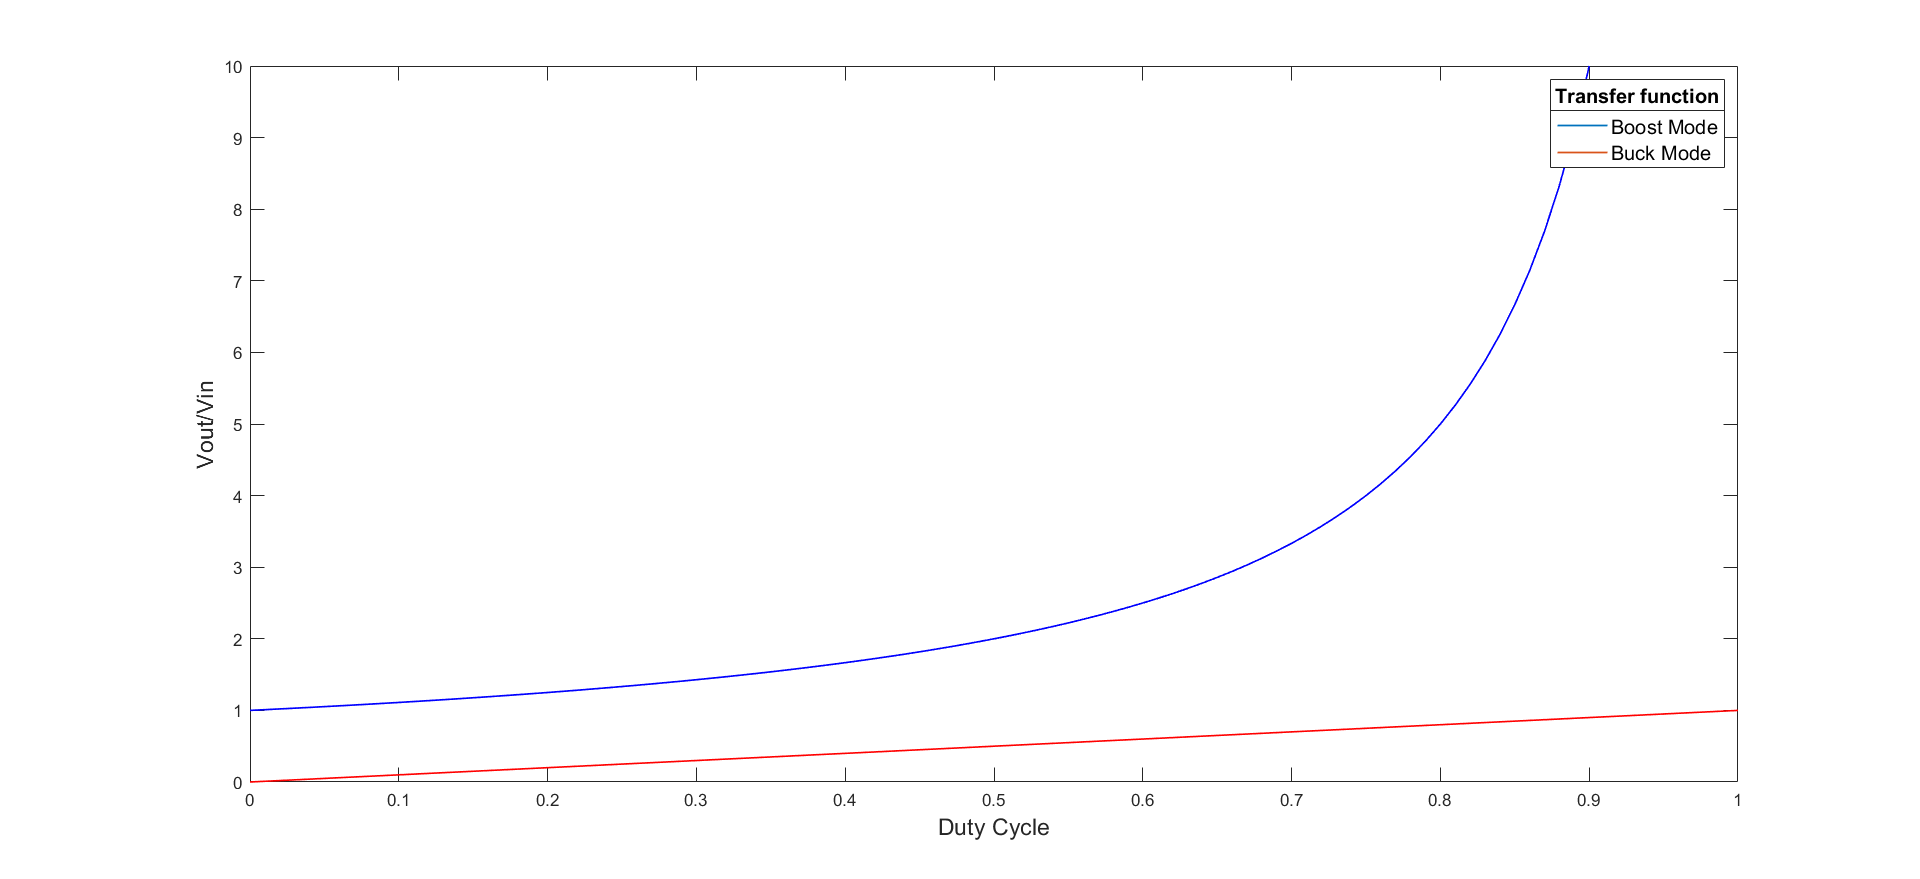
\includegraphics[width=\textwidth]{../Pictures/transfer_function_buck_boost_mode}
		\caption{Transfer function of buck mode and boost mode.}
		\label{fig:tfmodes}
	\end{minipage}
	\hspace{0.5cm}
	\begin{minipage}[b]{0.9\linewidth}
		\centering
		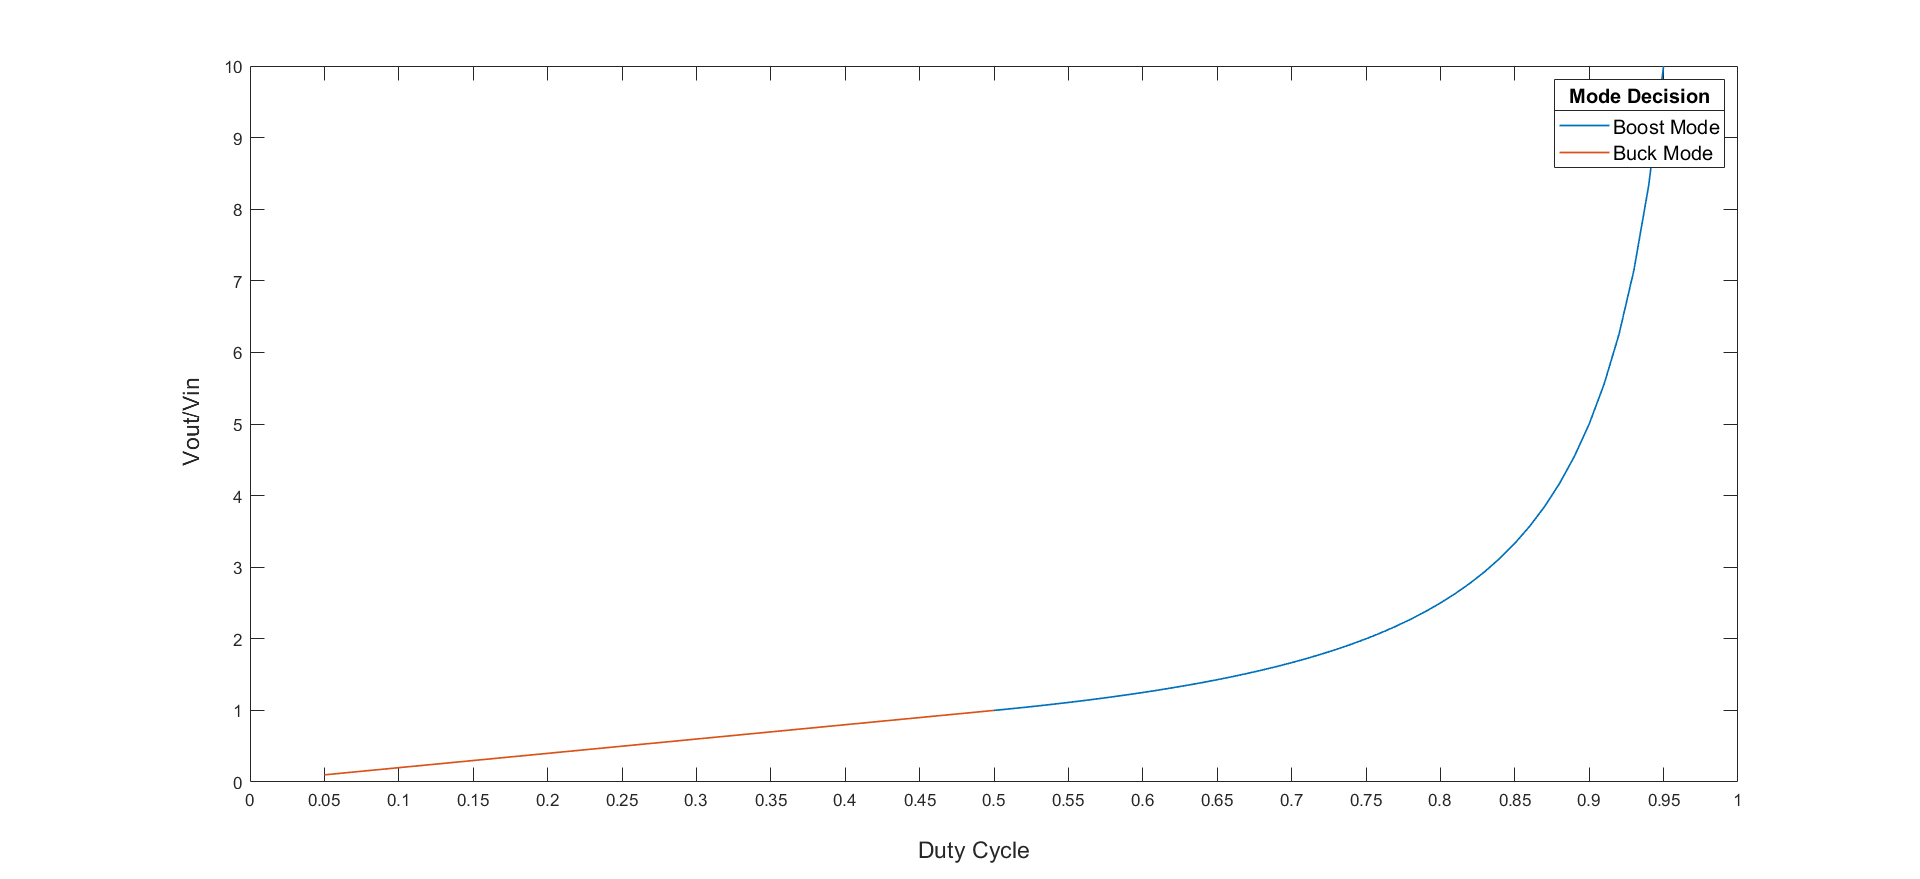
\includegraphics[width=\textwidth]{../Pictures/Mode_decision_duty_vs_gain}
		\caption{Mapping to decide the mode of operation.}
		\label{fig:modedecisionmapping}
	\end{minipage}
\end{figure}


The corresponding flow chart used for the implementation of the Perturb \& Observe algorithm is shown in figure \ref{fcfinal}.


\begin{figure}[H]
	\begin{center}
		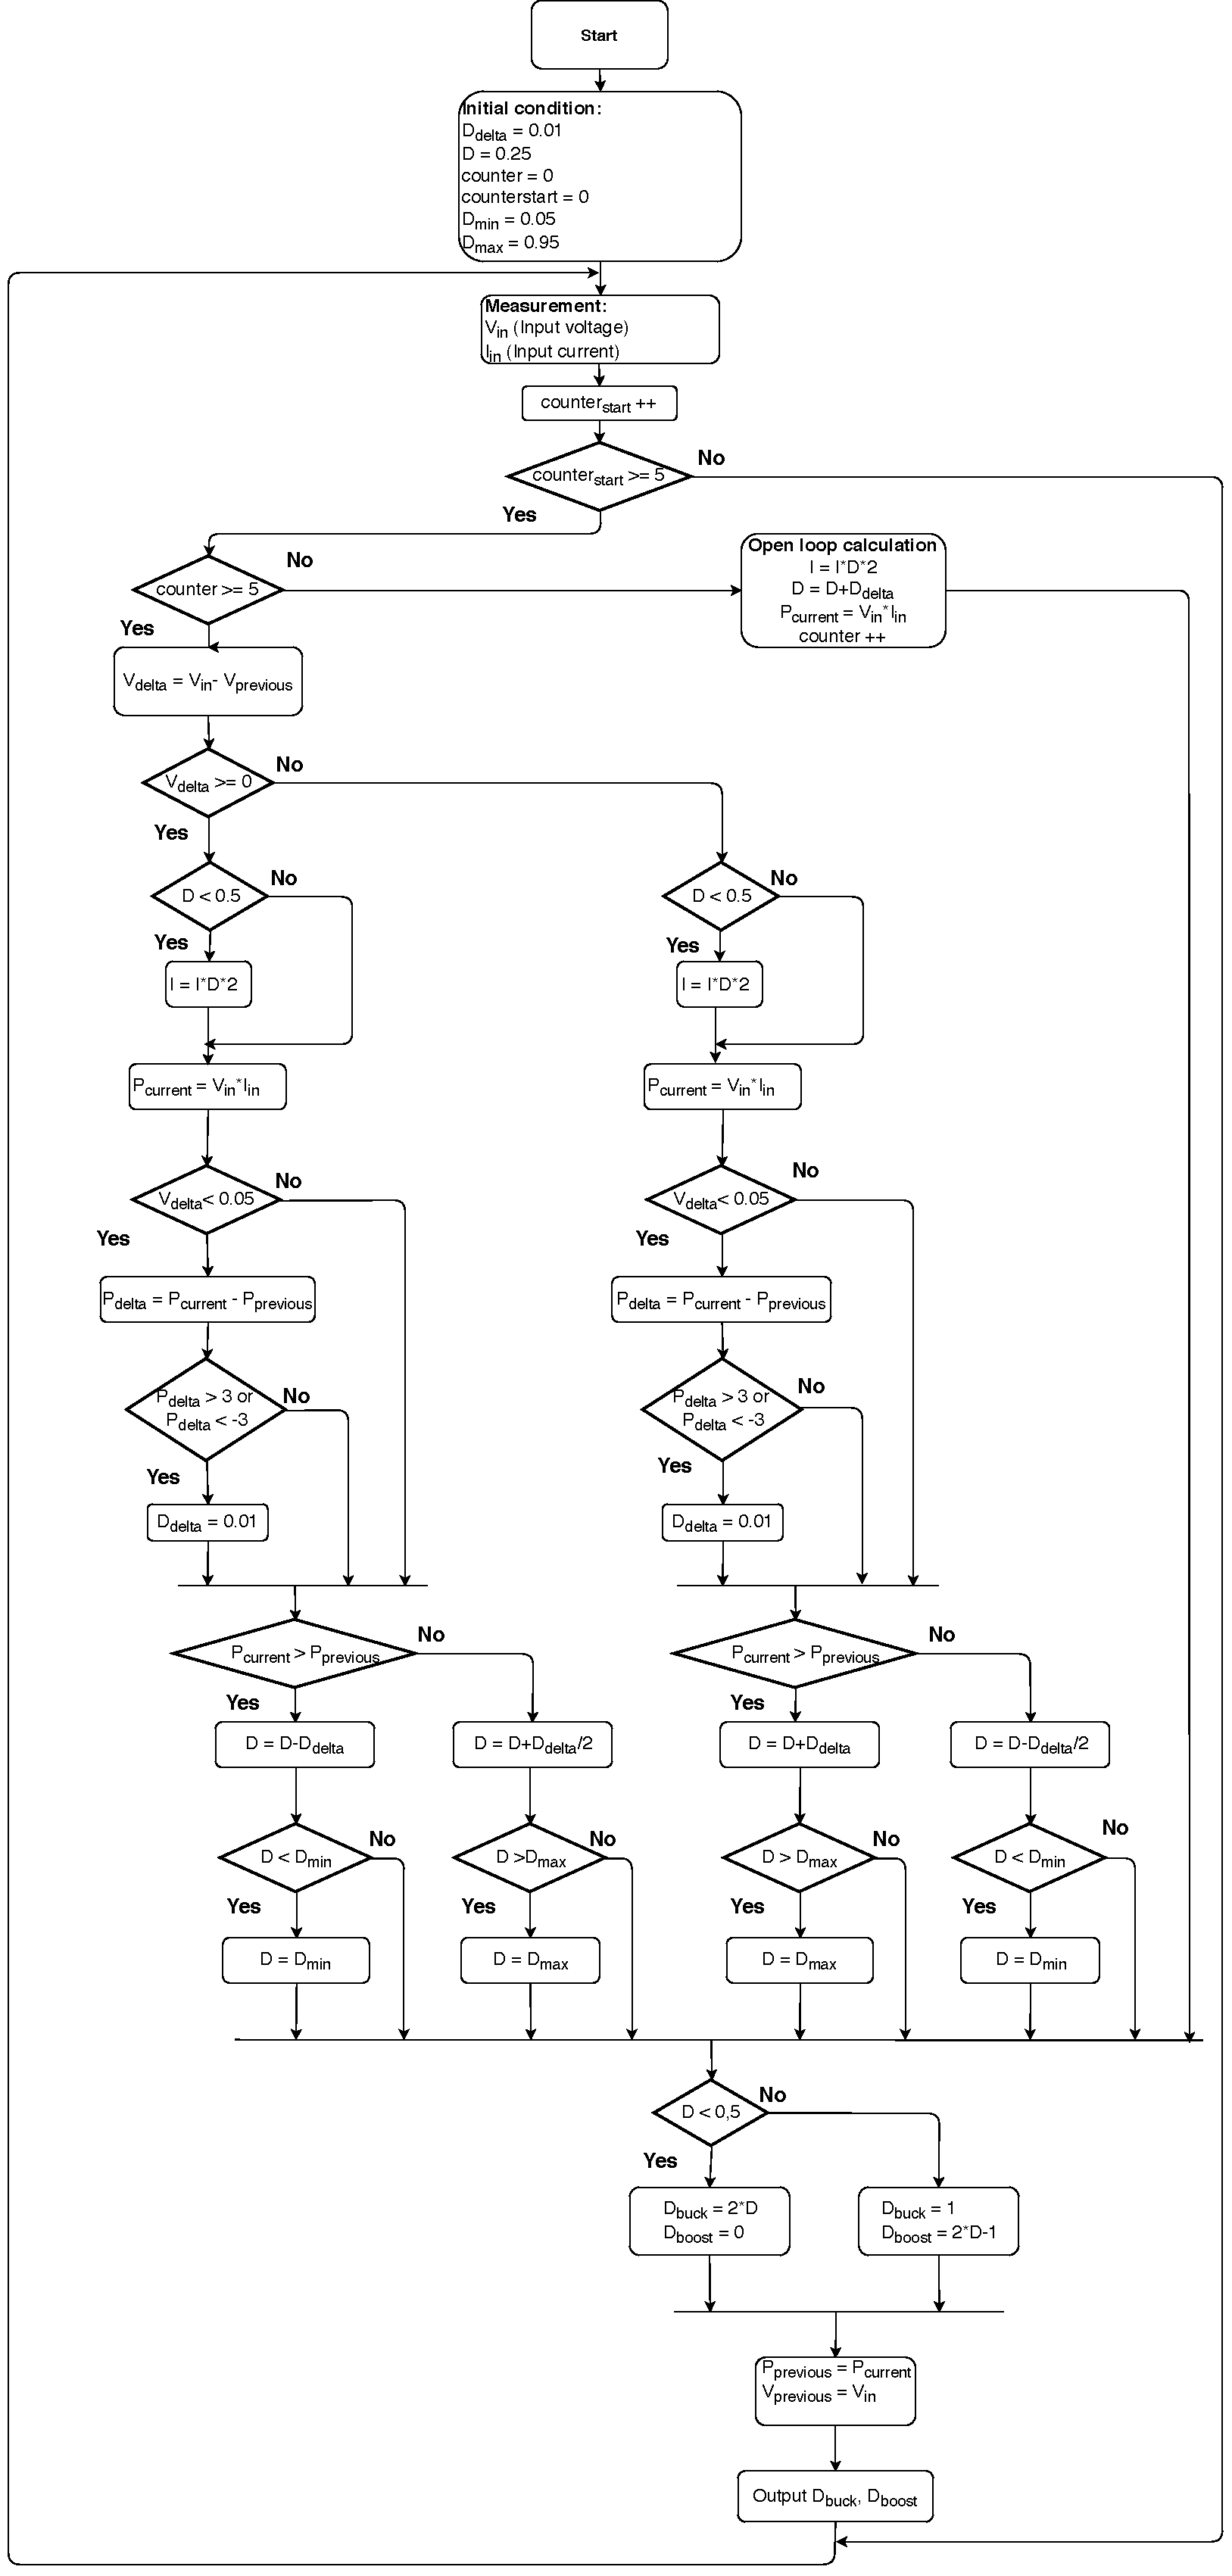
\includegraphics[width=0.8\textwidth]{../Pictures/P1/Flow_chart/2018_11_15_Flow_chart_MPPT_Buck-Boost_converter}
		\caption{Flow chart for the Perturb \& Observe algorithm.}
		\label{fcfinal}
	\end{center}	
\end{figure}

From the flow chart of figure \ref{fcfinal} it can be observed that the algorithm starts with initial conditions


It is important to notice from figure \ref{BD_POalgorithm} that the current measurement is carried out in the inductor instead of in the PV panel. This is done for possible future implementation of an outer PI control loop. For this reason, it is necessary to transform the measured current in order to get the corresponsing measurement for the PV module's current. This current transformation is just necessary in the case of buck mode as explained in section \ref{current_sensor}. The MPPT evaluates if the converter is working in buck mode and if it is it multiplies the measured current by the corresponding duty cycle $D_{buck}=2\cdot D$. In boost mode the current through the inductor corresponds to the PV module's current. 


Things to write in this section:
\begin{itemize}
	
	\item Initial conditions: enable the MPPT after 5Ts (50ms) to ensure that Vin has reached the open circuit voltage, counter = 5 to have some open loop measurements before starting the voltage evaluation, the system starts in buck mode (D=0.25) with fix variations of duty cycle (0.01), limits of duty cycle 0.05<D<0.95 to avoid problems in buck and in boost mode respetively. 
	\item Also mention the case when a change in irradiance takes place it's a good idea to reset the value of delta D to 0.01. This is because we are using variable step and when the system detects the change in irradiance it will keep the corresponding value of delta D which will be very small because the system already could have reached the MPP (variable step). 
\end{itemize}



